\documentclass{beamer}
\usepackage[utf8]{inputenc}
\usepackage[T1]{fontenc}
\usepackage[bulgarian]{babel}
\usepackage{alltt}

\useoutertheme{shadow}

\setbeamercolor{title}{fg=red!80!black}
\setbeamercolor{frametitle}{fg=red!80!black}

\usetheme[secheader]{Madrid}
\usecolortheme{crane}

%Тема 11.
%7.2 Constraints on Attributes and Tuples
%• Not-Null Constraints
%• Attribute-Based CHECK Constraints
%• Tuple-Based CHECK Constraints
%• Modification of Constraints
%• Giving Names to Constraints
%• Altering Constraints on Tables

\title[Дървовидни структури за многомерни данни в MySQL]{Дървовидни структури за многомерни данни в MySQL}
\author{Валентина Динкова, ф.н. 71112}
\institute{ФМИ}
\date{\today}
\begin{document}
\begin{frame}
  \titlepage
\end{frame}
%\begin{frame}
  %\frametitle{Съдържание}
  %\tableofcontents
%\end{frame}

\begin{frame}
  \frametitle{GIS и разширението на MySQL за пространствени данни}
\begin{itemize}
 \item Какво е \textbf{GIS} и какво е \textbf{OGC}?
\end{itemize}
\textbf{GIS} означава Географска Информационна Система и е един от най-очевидните примери за пространствени данни.
\newline
\newline
\textbf{OGC} (Open Geospatial Consorcium) е организация, която работи по стандартизирането на различни области на GIS.
Един такъв стандарт е и спецификацията за SQL, която определя разширение на SQL базирани релационни бази данни, което да използва GIS обекти и операции.
\end{frame}

\begin{frame}
 OGC работи в 4 важни области:
\begin{itemize}
 \item типове данни;
 \item операции;
 \item възможност да се подават като вход и да се извеждат GIS данни;
 \item индексиране на пространствени данни.
\end{itemize}
Друга важна област са метаданните
\end{frame}

\begin{frame}
\frametitle{Стандартът, използван от почти всички SQL бази данни с пространствено разширение, включително и MySQL}
\begin{center}
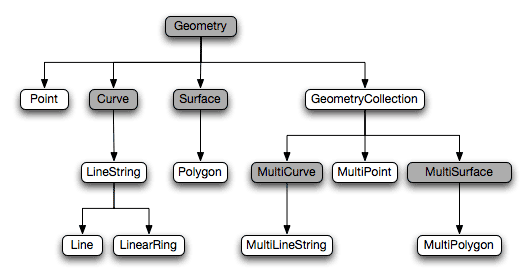
\includegraphics[width=60mm]{gis-datatypes.png}\end{center}
Типовете, отбелязани в сиво са абстракти и обекти от тези типове не могат да се създават.
\end{frame}

\begin{frame}
 \frametitle{Пространствени индекси}
\begin{itemize}
\item Пространствените данни могат да се индексират също както останалите данни в MySQL. Но за да бъде 
индексирането ефективно, се използва пространствен тип индексиране, реализирано чрез R-дървета. 
MySQL използва \alert{R-дървета с квадратично разделяне}.
\end{itemize}

%\begin{beamerboxesrounded}{R-tree splitting} 
%Quadratic method: Examine all the children of the overflowing node and find the pair of bounding boxes that would waste
% the most area were they to be inserted in the same node. This is determined by subtracting the sum of the areas of the
% two bounding boxes from the area of the covering bounding box. These two bounding boxes are placed in separate nodes,
% say j and k . The set of remaining bounding boxes are examined and the bounding box i whose addition maximizes the
% difference in coverage between the bounding boxes associated with j and k is added to the node whose coverage is
% minimized by the addition. This process is reapplied to the remaining bounding boxes [Gutt84]. This method takes
% quadratic time.
%\end{beamerboxesrounded}
\end{frame}


\begin{frame}[fragile]
\begin{beamerboxesrounded}{Създаваме таблицата $map\_test$, където $loc$ е пространствен атрибут}
\begin{alltt}
mysql> create table map_test
    -> (
    ->   name varchar(100) not null primary key,
    ->   \alert{loc  gepmetry not null},
    -> );
Query OK, 0 rows affected (0.00 sec)
\end{alltt}
\end{beamerboxesrounded}

\begin{beamerboxesrounded}{Добавяме данни}
\begin{alltt}
mysql> insert into map_test values ('One Two', point(1,2));
Query OK, 1 row affected (0.00 sec)

mysql> insert into map_test values ('Two Two', point(2,2));
Query OK, 1 row affected (0.00 sec)

mysql> insert into map_test values ('Two One', point(2,1));
Query OK, 1 row affected (0.00 sec)
\end{alltt}
\end{beamerboxesrounded}
\end{frame}


\begin{frame}[fragile]
\begin{beamerboxesrounded}{Ето как изглежда $map\_test$ сега:}
\begin{alltt}
mysql> select name, AsText(loc) from map_test;
+---------+-------------+
| name    | AsText(loc) |
+---------+-------------+
| One Two | POINT(1 2)  |
| Two Two | POINT(2 2)  |
| Two One | POINT(2 1)  |
+---------+-------------+
3 rows in set (0.00 sec)
\end{alltt}
\end{beamerboxesrounded}
\end{frame}

\begin{frame}[fragile]
\begin{beamerboxesrounded}{Заявка за проверка коя точка се съдържа в полигона}
\begin{alltt}
mysql> SELECT name, AsText(loc) FROM map_test WHERE
    -> Contains(
    -> GeomFromText('POLYGON((0 0, 0 1, 1 1, 2 0, 0 0))'),
    -> loc) = 1;
+---------+-------------+
| name    | AsText(loc) |
+---------+-------------+
| Two One | POINT(2 1)  |
+---------+-------------+
\alert{1 row in set (0.04 sec)}
\end{alltt}
\end{beamerboxesrounded}
\end{frame}

\begin{frame}[fragile]
\begin{beamerboxesrounded}{Сега създаваме пространствен индекс по атрибута $loc$}
\begin{alltt}
mysql> create spatial index ps_index on map_test(loc);
Query OK, 3 rows affected (0.01 sec)
Records: 3  Duplicates: 0  Warnings: 0
\end{alltt}
\end{beamerboxesrounded}
\end{frame}

\begin{frame}[fragile]
\begin{beamerboxesrounded}{И отново правим същата заявка}
\begin{alltt}
mysql>  SELECT name, AsText(loc) FROM map_test WHERE
    ->  Contains(
    ->  GeomFromText('POLYGON((0 0, 0 1, 1 1, 2 0, 0 0))'),
    ->  loc) = 1;
+---------+-------------+
| name    | AsText(loc) |
+---------+-------------+
| Two One | POINT(2 1)  |
+---------+-------------+
\alert{1 row in set (0.00 sec)}
\end{alltt}
\end{beamerboxesrounded}
\end{frame}

\end{document}